%% This is repurposed from `sample-sigconf.tex'
\documentclass[sigconf, nonacm, 11pt]{acmart}


\usepackage{graphicx}
\usepackage{hyperref}
\usepackage{cleveref}
\usepackage{tabulary}
\usepackage{soul}
\usepackage{subcaption}
\usepackage{algorithm}
\usepackage{algorithmic}
\usepackage{listings}
\usepackage{xcolor}
\usepackage{multirow}


%%
%% \BibTeX command to typeset BibTeX logo in the docs
\AtBeginDocument{%
  \providecommand\BibTeX{{%
    \normalfont B\kern-0.5em{\scshape i\kern-0.25em b}\kern-0.8em\TeX}}}

%%%%%%%%%%%%%%%%%%%%%%%%%%%%%%%%%%%%%%%%
% Useful reviewing/feedback annotations
\usepackage{ifthen}
\usepackage[normalem]{ulem} % for \sout
% \usepackage{xcolor}
% \usepackage{amssymb}

\newcommand{\ra}{$\rightarrow$}
\newboolean{showedits}
\setboolean{showedits}{true} % toggle to show or hide edits
%%\setboolean{showedits}{false} % toggle to show or hide edits
\ifthenelse{\boolean{showedits}}
{
	\newcommand{\ugh}[1]{\textcolor{red}{\uwave{#1}}} % please rephrase
	\newcommand{\ins}[1]{\textcolor{blue}{\uline{#1}}} % please insert
	\newcommand{\del}[1]{\textcolor{red}{\sout{#1}}} % please delete
	\newcommand{\chg}[2]{\textcolor{red}{\sout{#1}}{\ra}\textcolor{blue}{\uline{#2}}} % please change
}{
	\newcommand{\ugh}[1]{#1} % please rephrase
	\newcommand{\ins}[1]{#1} % please insert
	\newcommand{\del}[1]{} % please delete
	\newcommand{\chg}[2]{#2}
}

\newboolean{showcomments}
\setboolean{showcomments}{true}
%\setboolean{showcomments}{false}
\newcommand{\id}[1]{$-$Id: scgPaper.tex 32478 2010-04-29 09:11:32Z oscar $-$}
\newcommand{\yellowbox}[1]{\fcolorbox{gray}{yellow}{\bfseries\sffamily\scriptsize#1}}
\newcommand{\triangles}[1]{{\sf\small$\blacktriangleright$\textit{#1}$\blacktriangleleft$}}
\ifthenelse{\boolean{showcomments}}
%{\newcommand{\nb}[2]{{\yellowbox{#1}\triangles{#2}}}
{\newcommand{\nbc}[3]{
 {\colorbox{#3}{\bfseries\sffamily\scriptsize\textcolor{white}{#1}}}
 {\textcolor{#3}{\sf\small$\blacktriangleright${#2}$\blacktriangleleft$}}}
 \newcommand{\version}{\emph{\scriptsize\id}}}
{\newcommand{\nbc}[3]{}
 \renewcommand{\ugh}[1]{#1} % please rephrase
 \renewcommand{\ins}[1]{#1} % please insert
 \renewcommand{\del}[1]{} % please delete
 \renewcommand{\chg}[2]{#2} % please change
 \newcommand{\version}{}}
\newcommand{\nb}[2]{\nbc{#1}{#2}{orange}}

\definecolor{ibcolor}{rgb}{0.4,0.6,0.2}
\newcommand\iv[1]{\nbc{IB}{#1}{ibcolor}}
\usepackage{wasysym}
\newcommand\yesml[1]{\nbc{ML {\textcolor{yellow}\sun}}{#1}{mircolor}}

\definecolor{aycolor}{rgb}{0.2,0.4,0.2}
\newcommand\anil[1]{\nbc{Anil}{#1}{aycolor}}

\definecolor{ascolor}{rgb}{0.96,0.02,0.83}				% Alex's comments
\newcommand\alex[1]{\nbc{Alex}{#1}{ascolor}}

\definecolor{hccolor}{rgb}{0.21,0.54,0.84}
\newcommand\hc[1]{\nbc{HC}{#1}{hccolor}}

\definecolor{ideacolor}{rgb}{1.0,0,0.5}
\newcommand\idea[1]{\nbc{IDEA}{#1}{ideacolor}}

\definecolor{mccolor}{rgb}{0.2,0.2,0.6}
\newcommand\mc[1]{\nbc{Meta}{#1}{mccolor}}


\definecolor{abstractcolor}{rgb}{0.0,0.5,1.0}
\newcommand\rabstract[1]{\nbc{ABSTRACT}{#1}{abstractcolor}}

\definecolor{introcolor}{rgb}{0.0,1.0,0.5}
\newcommand\rintro[1]{\nbc{INTRO}{#1}{introcolor}}

\definecolor{papercolor}{rgb}{1.0,1.0,0.0}
\newcommand\rpaper[1]{\nbc{PAPER}{#1}{papercolor}}

\definecolor{multicolor}{rgb}{1.0,0,0}
\newcommand\rmulti[1]{\nbc{MULTI}{#1}{multicolor}}

% Todo Command
\definecolor{todocolor}{rgb}{0.9,0.1,0.1}
\newcommand{\todo}[1]{\nbc{TODO}{#1}{todocolor}}

% Todo Command
\definecolor{qcolor}{rgb}{0.2,0.0,0.9}
\newcommand{\ques}[1]{\nbc{Ques}{#1}{qcolor}}

%%%%%%%%%%%%%%%%%%%%%%%%%%%%%%%%%%%%%%%%

%%
%% end of the preamble, start of the body of the document source.
\begin{document}

%%
%% The "title" command has an optional parameter,
%% allowing the author to define a "short title" to be used in page headers.
\title[How To Build Your Disaggregated Memory System]
{How To Build \\Your Disaggregated Memory System} % 
\author{Anil Yelam}
% \affiliation{
%  \institution{UC San Diego}}
\email{ayelam@ucsd.edu}



\begin{abstract}
\end{abstract}
\maketitle

\section{INTRODUCTION}
\label{sec:intro}

\begin{figure*}[h!]
    \centering
    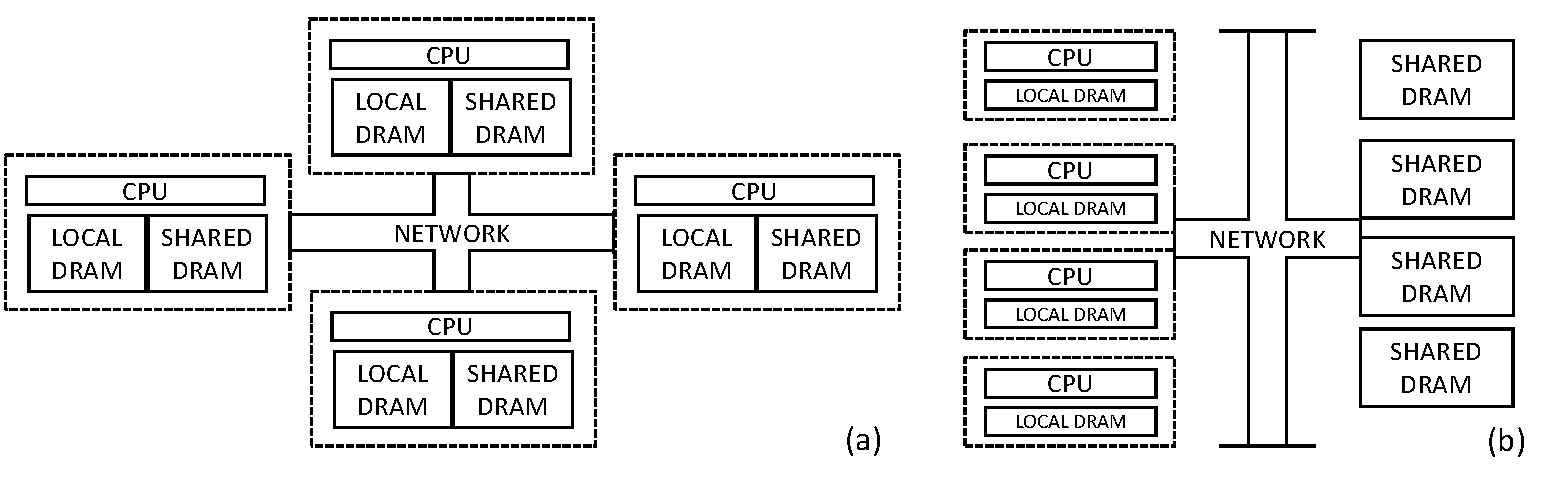
\includegraphics[width=.9\linewidth]{fig/architecture.pdf}
    \caption{(too big?) Shows (a) software-disaggregated 
    architecture where disaggregated memory is pooled from 
    traditional servers as opposed to the (b) hardware-disaggregated
    design where most memory is decoupled in hardware.}
    \label{fig:architecture}
\end{figure*}

With the tremendous growth of computing in the past two 
decades, applications have become both data-intensive 
and latency-sensitive, which gave rise to in-memory 
computing in lieu of going to the disk. 
This led to memory-intensive 
applications whose memory needs on a server outweigh the 
processor needs, introducing a skew in resource usage.
However, traditional servers come with fixed processor 
and memory resources that does not allow dynamically
resizing memory. This was generally solved by swapping 
to disk but disk speeds were really slow compared to memory 
affecting performance. 
At the same time, the diversification of computing usecases 
introduced a high heterogeneity of applications (e.g., cloud 
computing) with varying memory needs in proportion to 
the CPU, leaving some of the traditional servers in a data center  
with underutilized memory and others with not enough; the result
being inefficient memory utilization in the cluster and hence,
increased cost of ownership. Decoupling memory would allow 
applications to be more elastic in their memory usage and 
improve the memory utilization of the cluster at the same time.
Memory disaggregation involves such (logical or physical) 
decoupling of memory resources in a cluster from other 
(processor) resources. 
% \anil{there are other benefits to memory disaggregation...}

One way to alleviate memory pressure is to scale out and 
build a distributed application that runs on multiple nodes and 
adjust itself to the memory restrictions on the individual 
nodes. Indeed, there are many platforms that provide distributed 
memory management for such applications like distributed key-value 
stores~\cite{Ousterhout2010,Lim2012,Novakovic2016,Kalia2015},
distributed shared memory (DSM) 
systems~\cite{treadmarks,dsm1,farm,gam}, etc. These systems 
provide a globally accessible interface for all servers where  
the focus is on providing fine-grained memory sharing and 
a reasonable consistency model for distributed applications. 
An alternative is to extend the private memory space 
of (single-node) applications a la 
remote swapping systems~\cite{gms,cashmere} that transparently
swap application pages to remote memory without any notion 
of sharing across servers (i.e., their memory 
consistency model stops with cache coherence protocols on a 
single server). In this report, we focus 
on the latter kind where the stress is more on perfomant 
remote access mechanisms and efficient memory management for 
individual applications and less on memory sharing and 
consistency across servers.

As the networks become faster and technologies such as 
RDMA~\cite{farm,rocev2} arrive to commodity clusters, 
the remote access latencies are inching closer to native 
DRAM latencies (which, on the contrary, are nearing 
saturation~\cite{Aguilera2017}), making remote memory more 
accessible for applications, performance-wise~\cite{netdisagg}. 
Consequently, there has been a renewed interest in 
recent years in building remote memory 
systems~\cite{infiniswap,zswap,leap,fastswap,
legoos,kona,aifm,semeru,remregions,literdma}.
Traditional way of memory disaggregation is to pool/track  
unused memory across the cluster in software 
and use it to complement memory on the memory-hungry servers.
This is still popular with work on remote swapping systems 
continuing to this day~\cite{infiniswap,fastswap,zswap,leap}.
The other, more recent approach is to disaggregate the memory 
in hardware and where all the memory is decoupled from compute
and is made available to the compute nodes via 
the network~\cite{legoos,bladedisagg1,sonuma}. 
(we use the terms \textit{remote} or 
\textit{disaggregated} memory synonymously to refer 
to all the memory 
available for shared usage of the cluster whether it is 
pooled in software or hardware). 

In both cases, building a system 
that exposes and manages such disaggregated memory face  
similar design challenges. First, the system should decide on
the right interface to expose this memory; for example,
to either be transparent and avoid any application changes, 
or to be more expressive and provide richer functionality and 
exploit app semantics for performance. Moreover, remote access 
latencies are still an order-of-magnitude worse than local, so the 
system should implement on performance optimizations like caching 
or at the least, enable applications to implement such optimizations. 
While providing reasonable programming model and performance
for a wide range of applications, it should also work towards 
efficiently managing the cluster memory behind the scenes and 
maintain good memory utilization.

In this report, we explore in detail, the above design 
challenges of building a system for disaggregated memory, 
in addition to some more that is expected of a holistic 
system e.g., fault tolerance, reliability, security and 
isolation, etc. through the lens of recent 
disaggregated/far memory systems. 
Through this analysis, we hope to 
highlight the trade-offs involved with various design 
considerations. We end with a discussion of remaining 
challenges in the system design e.g., \todo{}.

\section{Background}
\label{sec:background}

% \vspace{5pt}
% \noindent \uline{Historical work.}
% Very early work on improving cluster memory 
% utilization ~\cite{gms,cashmere,treadmarks,dsm1} 
% sticked to traditional server architectures and focused on 
% software-based memory pooling across the cluster and exposing it 
% to applications in (mainly) two different flavors. 
% Distributed shared memory (DSM) systems~\cite{treadmarks,dsm1} 
% provide a global shared address space for writing distributed 
% applications, where the address space is globally accessible 
% from all the servers. These systems can then transparently 
% back subsets of address space (at different granularity) with 
% physical memory from different servers across the cluster, and 
% therefore have the flexibility of optimizing cluster memory 
% utilization. Other systems like GMS~\cite{gms, cashmere} just 
% focus on extending the address space of individual applications 
% without any notion of sharing across servers (i.e., their memory 
% consistency model stops with cache coherence protocols on a single 
% server). These systems merely back or complement local DRAM with 
% unutilized memory from other servers using the paging mechanisms 
% in the operating system, usually by providing remote memory as 
% another block device to swap to. DSM systems 
% provide shared memory (along with some consistency model) which 
% makes distributed programming easier but they may require 
% applications be rewritten using their memory model. Conversely, 
% remote paging systems aim to be more backwards-compatible and 
% leave the complexity of building distributed applications 
% (if needed) to the higher layers. These early systems however 
% hasn't seen adoption (perhaps?) because remote memory latencies 
% were still far higher for tenable application performance. 
% (DSM though had even more challenges due to overheads in 
% ensuring consistency that get amplified with slow networks).
% \vspace{5pt}
% \noindent \uline{Recent proliferation in this space.}
As the remote access latencies come closer to native 
DRAM latencies (which, on the contrary, 
are nearing saturation~\cite{Aguilera2017}),
writing applications with such accesses 
in the critical path is looking feasible, 
performance-wise~\cite{netdisagg}. 
Consequently, there has been a lot of RDMA-inspired remote 
memory system building in recent years, including a renewal in
DSM~\cite{farm, gam,dspm,ltdsm} and Remote 
paging~\cite{Lim2012,bladedisagg1,infiniswap,zswap,fastswap,leap} 
systems. While the remote paging systems provide native virtual memory 
interface (i.e., memory access through load/store ops on cached 
local pages from remote memory) to applications, 
other new interfaces for remote memory were proposed that 
sacrifice application transparency in favor of performance 
due to either the simplicity of 
implementation~\cite{remregions,literdma} (light-weight runtime 
means less performance overhead in the critical access path) or 
benefits from application hints~\cite{aifm}; 
conversely, these interfaces require app modifications but
enable applications to distinguish between local and remote 
memory accesses and be smart about it e.g., use far-memory 
aware implementations~\cite{Aguilera2019,semeru}.

Most systems for disaggregated memory target clusters with 
traditional (commodity) servers where memory is collocated 
with processors and there is no special hardware support.
Traditional hardware cannot access remote memory directly 
and hence usual solutions has to proxy it  
through local memory by caching remote data and resorting to 
software to fetch remote data on a cache miss. To avoid 
this overhead, some systems introduce special hardware 
like a remote memory controller~\cite{sonuma} or a 
cache-coherent FPGA~\cite{kona} to plug into 
the local cache hierarchy and handle remote accesses through 
the hardware. And finally, as an alternative to traditional 
server model, there were proposals for new 
hardware architectures where memory is decoupled and pooled
at a hardware-level, and some systems targeting such 
disaggregation~\cite{sonuma,bladedisagg1,legoos} as well. 
In this report, we will look at many of these systems to 
provide an informed view of disaggregated system design.

\section{Memory Disaggregation}
Memory disaggregation aims to decouple the available compute 
and memory resources in the cluster and allow for independent 
allocations of these resources regardless of where a job 
is placed in the cluster. This means, the OS/runtime 
that's running the job should provide a platform to 
expose/give access to potentially all the memory 
available in the cluster. Ideally, it should hide the complexity 
of setting up and accessing remote memory (e.g., RDMA 
connection and queue pair management) and expose an
easy-to-use interface for working with remote memory.
At the same time, it should trade-off the properties 
of the interface with decent performance guarantees 
and other requirements from the system like resource 
sharing and isolation across applications. At a high 
level, the platform is a distributed system consisting 
of a client-side (compute-side) component (a runtime 
that exposes the memory interface and acts as an agent 
on each compute node), the server-side (memory) component 
(to manage memory on the server) and an 
interconnect over which these components 
interact to provide an abstraction for shared cluster memory.
It may optionally include other cluster resources for 
global memory/metadata management. \todo{figure?} 

\subsection{Target Architecture}
Proposed solutions for memory disaggregation target two 
different kind of cluster/memory architectures based on
existing technologies or technologies that are expected
to be available in the near future; we look at system
design targeting both these architectures (shown in 
Figure ~\ref{fig:architecture}).

\vspace{3pt}
\noindent \uline{\textit{Software-disaggregated.}}
Some systems~\cite{gms,cashmere,infiniswap,remregions,leap,zswap} 
target the traditional homogeneous 
datacenters with monolithic servers as the basic 
deployment unit, connected to each other by low-latency 
network interconnects like Infiniband or RoCE. Each 
unit hosts both compute and memory resources and the 
software provides an interface to remote memory 
on other nodes. Local memory is prioritized for 
local jobs and unutilized memory on all the nodes 
can be pooled and presented to the cluster as 
remote/disaggregated memory, which could be static 
or vary in capacity over time. 

% In this case, the fault domain is the 
% single server unit i.e., if a component on a server fails, 
% the whole unit usually fails. (Although solutions like Zombieland\cite{zombieland} 
% were proposed to decouple CPU from memory failures and 
% vice versa in monolithic servers.\todo{confirm}))

\vspace{3pt}
\noindent \uline{\textit{Hardware-disaggregated}}
Other systems~\cite{kona,aifm,fastswap,semeru}, like LegoOS~\cite{legoos}, target a hardware-disaggregated 
architecture where (most of the) 
memory nodes are detached from the compute nodes and 
made available through the network. The memory node 
can be a traditional monolithic server with limited 
compute and stuffed with DRAM~\cite{fastswap} or 
each DRAM unit itself directly-attached to a memory 
controller and network interface~\cite{legoos}. 
Even in a purely disaggregated setup, however, 
it is generally assumed that each compute node has 
a small amount of local memory and vice 
versa.~\cite{legoos,kona}

% While the 
% former is more amenable for existing deployments, the 
% latter requires newer technologies like Intel 
% OmniPath~\cite{omnipath} to attach DRAM to the network 
% without a processor.

% The latter, however, is also more fault tolerant as each 
% DRAM unit is failure-isolated and does not affect other 
% units.

In both architectures, compute servers use local memory 
to run the OS and other runtime essentials for exposing remote 
memory\footnote{we use the terms remote or disaggregated 
memory synonymously to refer to all the memory 
available for shared usage of the cluster in both 
architectures}, and only use remote memory for the applications. 
There are many reasons for this choice. 
First, without local DRAM, all the memory 
accesses would be remote and the memory controller should 
possess the knowledge and capability to fetch remote memory 
directly without any help from software; such complex "control 
path" knowledge would need either a "smart" memory controller 
(e.g., RMC in soNUMA~\cite{sonuma}) or some other smart 
hardware (e.g., ccFPGA in Kona~\cite{kona}) next to it. 
Even these solutions do not put OS on remote memory and 
and maintain local DRAM to exploit cache locality as remote 
accesses are still an at least an order of magnitude higher 
than local.

\anil{explain other benefits like fault tolerance?}

\section{Design}
\label{sec:design}
We look at various considerations that guide the design of a 
disaggregated system and for each of them, we discuss why it 
matters, how previous systems have (not) treated it, are there 
going to be trade-offs with others, etc. 

\subsection{Programming Model}
A key question for a disaggregated system is how it 
chooses to expose the memory (both local and remote) of the 
cluster to the applications running on it. Below, we talk about 
various aspects of the interface, while referring to 
previous systems (Table \ref{tab:interfaces}).

\subsubsection{Transparency}
Does the app (need to) know whether an access is local or 
remote? Does it require a rewrite of applications or can 
existing applications port to it with minimal or no effort?

\vspace{3pt}
\noindent \uline{Virtual memory-based transparency.}
In a traditional (x86) server, access to local memory is 
provided through the virtual memory abstraction using 
the load/store-style instructions on virtual addresses 
whose translation is handled by hardware (TLB, MMU) and 
managed by the OS. The same virtual memory abstraction can 
be extended to remote memory as well. The abstraction 
allows the actual pages to be backed my any device 
(disk, remote memory, files, etc.) from where they can 
be fetched when accessed by hooking into the page fault 
handler. The main benefit is complete backwards-compatibility 
and language-agnosticism where all the applications 
targeting x86 hardware can utilize  
remote memory without a single line of code change. The flip side 
is that this interface is rigid (it cannot be extended like a
regular API) and kernel-based and so doesn't allow any 
app-specific information to percolate into the runtime and 
limits its performance optimizations, as we will see in 
section \ref{sec:performance};


Due to its complete transparency, it has been the 
go-to interface for all the \textit{remote paging} systems 
from the old~\cite{gms,cashmere} that continue to this
day~\cite{infiniswap,fastswap,zswap,leap}.
These systems target traditional servers 
(software-disaggregation) and provide remote memory as a swap 
space by hooking into the virtual memory manager in the kernel.
In the hardware-disaggregated setting, LegoOS~\cite{legoos}, a 
operating system designed for this setting, provides a similar 
interface for disaggregated memory. LegoOS models local DRAM as
next level \textit{virtually-indexed} cache and moves address 
translation hardware (TLB, paging hardware, etc.) to the memory
nodes. Similar to page-faults, cache misses are handled in 
software when the remote pages are fetched into local DRAM.
This interface also allows the whole application memory 
(code, stack and heap) to be in remote memory as all of it 
can be transparently paged out.
% restricts the granularity of dealing remote data to pages. 
% While smaller page size is better 
% from a remote memory perspective (for accurately tracking 
% applications memory accesses to provide better caching and 
% avoid moving around unnecessary data), it would worsen local 
% memory performance as it increases TLB faults.

Kona~\cite{kona} is a recent work that proposes a hardware-based 
implementation for this interface that avoids software overhead in
handling page faults/cache misses. It proposes hardware primitives 
that assist with trap remote memory accesses at the memory controller 
hardware and fetch them from the remote memory. In an example 
implementation, Kona uses cache-coherent FPGA that is connected to 
CPU using interconnects like CXL\cite{ccix}. This 
interconnect provides the FPGA with visibility to all the memory 
accesses through cache coherence protocol and routes all remote 
accesses through this hardware, which implements the runtime. 
This approach however requires special hardware.

\vspace{3pt}
\noindent \uline{Language-based Transparency.}
Without special hardware support like Kona~\cite{kona}, 
only a kernel (paging) based implementation can provide 
the completely transparent memory interface that can be 
exploited by all the traditional applications
without application changes. However, kernel-based 
implementations suffer from I/O amplification and 
incomplete information on memory access 
patterns because the data tracking and movement granularity 
(fetching remote data) is restricted by the virtual memory 
system i.e., the kernel must fetch the entire page (4 KB) 
just to access even a small object. And the simplicity  
of the virtual memory interface 
(malloc and load/store) also means that it makes it 
harder to provide application-specific semantics or 
hints to the runtime for optimized implementation. 
For example, similar to NUMA-aware data 
structures, data structures designed with far memory 
awareness might perform better than traditional ones 
running on a memory-transparent interface~\cite{Aguilera2019}. 

To imbibe application semantics into the runtime, systems 
like AIFM (Application-Integrated Far Memory)~\cite{aifm} 
and Semeru~\cite{semeru} opt for implementing their runtime in 
Userspace and bypass the kernel. Since native addresses can 
only point to local memory, another level of indirection 
is needed to address memory in order to hide remote memory
and retain some transparency. AIFM provides such indirection 
using C++ smart pointers while Semeru 
uses Java virtual addresses. This indirection also lets 
the runtime to track accesses at a much finer object 
granularity to perform more precise hotness tracking 
(leading to better cache eviction policies) and avoid 
data amplification. The indirection may however add some 
performance overhead in critical path compared to native 
memory accesses. Also, user space runtimes cannot place entire 
memory remotely
(e.g., local process segments like stack and code has to be in 
local memory) which may offset the decoupling benefits of 
disaggregated memory (e.g., scalability).

Programming languages provide inbuilt implementations of 
common data structures like lists and hash tables either as 
language primitives or as a part of standard libraries. 
One way to take achieve app-runtime codesign while preserving 
transparency (i.e., no or minimal changes) for applications 
is to modify just these implementations under the hood to be 
far memory-aware. AIFM, for example, provides remoteable 
alternatives to standard data structures that provide access 
hints to the prefetcher or offload data-intensive operations 
like copy, aggregation, etc. to the memory server. Similarly,
language runtimes can optimize their implementation around 
remote memory. For example, remote access latency can 
be hidden by maintaining lightweight threads and running other
threads while some thread waits for remote data~\cite{aifm}.  
Similarly, garbage collectors in managed runtimes like Java
can be optimized to target remote memory by offloading the 
data-intensive parts like object traversal to the memory 
servers~\cite{semeru}.


\vspace{3pt}
\noindent \uline{No Transparency.}
Some interfaces provide remote memory through a custom APIs 
(usually implemented as a set of library or system calls) that 
are not limited by the requirement to abstract away remote 
memory and to be backwards-compatible. Without such a 
limitation, the API can choose to be very expressive.
These APIs generally provide methods/calls for allocating and 
accessing remote memory, and in some cases, synchronization or 
transactional primitives for sharing memory across machines. 
Performance optimizations like caching are generally left to 
the applications. With non-transparent interfaces, however,
the choice of what goes in local vs remote memory is left to 
the application. Since local memory is inflexible, leaving 
this choice to applications may hurt the ability of the 
runtime to efficiently perform memory decoupling and other 
goals of memory disaggregation.

% Examples for this abstraction are PGAS-style global memory
% exposed through read/write calls on each address. 
% Recent distributed computing platforms like FARM~\cite{farm} 
% and GAM~\cite{gam} employed this abstraction to 
% provide a unified address space partitioned and owned 
% across all the available nodes. Remote Regions~\cite{remregions} 
% and LITE Memory regions~\cite{literdma} expose 
% kernel-based remote memory APIs in an effort to provide a
% higher-level abstractions for RDMA.
Examples for such interfaces include Remote Regions~\cite{remregions} 
and LITE Memory regions~\cite{literdma} that expose an expressive
kernel-based remote memory API in an effort to provide a 
higher-level abstraction for RDMA.
These systems provide a namespace for (contiguous) memory 
segments (of arbitrary sizes) exposed by machines across the 
cluster and allow client apps to bind to these segments, 
and read/write through the ioctl stubs. The more expressive 
interface gives them the flexibility to expose various 
additional operations like the RPC support in LITE and 
caching/prefetching hints in Remote Regions. 
These interfaces however keep it low-level and does not take 
all the complexity of careful memory management and performance 
optimizations (next section) and limit themselves to naming 
and providing fast access to remote memory segments. Other 
complex systems can certainly use these interfaces 
(e.g., LegoOS uses LITE as the interconnect) for ease of 
implementation. Other (user space) examples include the 
transactional read/write semantics provided by
remote memory by recent distributed computing platforms like
FARM~\cite{farm} and GAM~\cite{gam}.

% Particularly, user space runtimes like 
% AIFM or Semeru can use these interfaces to complement them 
% and provide a complete system that supports sharing and 
% isolation.


\subsubsection{Generality} 
Is the exposed interface (ABI/API) 
general enough for adoption across wide range of 
platforms/applications, or does it favor a particular app 
above or particular runtime below, potentially falling out 
of favor with new kinds of apps/hardware? For example,
interfaces provided through the kernel-based runtimes 
(either transparent ones based on virtual memory or 
non-transparent ones exposed through ioctl stubs) cater to  
all the applications regardless of the language they are 
written in. In addition to being language-specific, user space 
runtimes~\cite{aifm,semeru} only support remote memory 
access/management for a single application and hence cannot 
co-ordinate sharing (and isolation) of available remote 
memory among multiple applications. Such sharing requires 
mediation of the kernel, at least in the control path.


\subsubsection{Ease of programming.} 
How easy is it for applications to program with this interface? 
When working with remote memory, this depends on how much of the 
complexity of implementation does the interface and the runtime 
hide away from the application. Naturally, transparent interfaces
are usually the easiest to program with. Of the non-transparent 
ones, the complexity may vary depending on how high-level or 
low-level the abstractions they provide are. As pointed out in
\cite{Aguilera2017}, adding two variables in disaggregated memory
would be a simple operation with virtual memory interface 
(*c = *a + *b). With non-transparent but still high-level 
abstractions like LITE~\cite{literdma}, we need to first open/map
the remote memory as LITE region, read variables using \textit{
LT\_read()} and write the result back using \textit{LT\_write()}.
Doing the same with using RDMA would be even more complex with 
setting up queue pairs and memory regions, and reading/writing 
data by posting work requests. A common but imperfect metric is 
to compare number of lines of code (LOC). For example, Both
LITE~\cite{literdma} and Remote Regions~\cite{remregions} show 
two orders of magnitude reduction in LOC compared to RDMA-based 
implementation. \todo{figure showing a typical transparent vs 
non-transparent interface}
    
\subsubsection{RPCs.} Some operations may be 
highly sensitive to remote accesses (like graph traversal) 
and can benefit immensely from having the operation 
run on a memory server (either in hardware or software 
depending on the memory server architecture). To support this,
interfaces allow applications to register/invoke methods on 
the remote node, such as function shipping in FaRM~\cite{farm}, 
AIFM Remote Devices~\cite{aifm}, LITE RPC~\cite{literdma}, etc.
Their scope is generally limited to simple (pre-determined) 
operations on few memory locations known to be on the memory 
server. Depending on server capabilities, they may not be
entirely feasible in hardware disaggregated scenarios.
Perhaps a middle ground is find a set of hardware primitives 
(as in~\cite{Aguilera2019}) for common remote side operations and 
expose only these set as RPCs through platforms like 
Storm~\cite{storm} and Strom~\cite{strom} that enable  
implementing these RPCs on the remote NICs.    

\subsubsection{Sharing across nodes.} Does the interface allow 
sharing the disaggregated memory across multiple nodes? If so, 
what kind of consistency model does it provide/allow? What 
kind of synchronization primitives does it provide (basic 
or advanced)? If sharing is to be supported for transparent virtual 
memory interface, it should provide same semantics as current 
cache coherence protocols on the entire address space but 
providing such strong consistency model across the network 
is still infeasible (even recent DSMs~\cite{farm,gam} based on 
RDMA do not attempt it); none of the major (transparent) systems~\cite{infiniswap,legoos} provided this support, perhaps for 
this reason. Non-transparent ones like 
Remote Regions~\cite{remregions} and LITE~\cite{literdma} provide
support for mapping the same region in multiple servers along with
basic synchronization support like barriers and mutexes for 
synchronizing their accesses, but no consistency on reads/writes. 
Sharing generally disallows caching and delayed write-backs,
both of which are critical to making performance of remote memory 
feasible for applications, as we will see in the next section.
\todo{needs work}.

\subsection{Application Performance}
\label{sec:performance}
When running on a disaggregated system, we ideally expect 
no or minimal degradation in application performance 
when compared to local memory performance. Depending 
on the application, one can look at its job completion time, 
throughput or tail latencies as a proxy for performance. 
(Although, metrics like total cost of ownership (TCO) are 
more holistic and account for things like memory 
utilization across the cluster, special hardware costs, etc.
but they are harder to measure?). In this section, we 
look at various factors that affect the memory performance,
through these metrics.


\subsubsection{Caching}
Remote accesses across the network today are still on 
the order of 10-100x slower with depending on the 
networking stack and interconnect, so application 
performance would be terrible if all accesses were 
to be remote~\cite{netdisagg}. Fortunately, most 
applications exhibit spatial and temporal locality 
in accesses which can be exploited by caching 
remote data, and as such the quality of caching can 
greatly affect the performance. Depending on the 
interface exposed, the runtime may choose to do 
caching or leave it to the application itself. 
Custom interfaces can enable application-specific 
caching hints. For example, AIFM~\cite{aifm} allows 
applications to exclude caching specified data and 
avoid cache pollution. 

\vspace{3pt}
\noindent \uline{Cache Block Size.} Fetching remote data in 
bigger chunks will help exploit spatial locality 
however it also runs the risk of bringing in redundant data 
and polluting the cache, so it needs to be properly 
balanced for the best cache hit ratio. Traditional
virtual memory-based approaches cannot go lower than 
the (4KB) page sized blocks as they hook into kernel 
paging; While LegoOS~\cite{legoos} and Kona~\cite{kona} 
escaped this fate through hardware modifications, 
other systems like AIFM~\cite{aifm} moved to user 
space implementations. Kona evaluates the effect of 
cache block size on the performance of Redis database 
and determines 1KB to be optimal, which is conveniently 
closer to the page size. However, Kona does not do any 
advanced prefetching (like Leap~\cite{leap}) which, in 
combination with smaller block sizes, may perform better 
than exploiting crude spatial locality with bigger blocks.
Block size also effects eviction policies like LRU (which
most systems use) as smaller blocks mean a larger number 
of blocks that need to be monitored for finding eviction
candidates. 

\vspace{3pt}
\noindent \uline{Prefetching.}
Prefetching remote data proactively can bring in 
correct pages into the cache and avoid cache misses 
in the critical path. Runtimes can use a transparent 
prefetcher that identifies access patterns and predict 
future accesses and/or they can provide prefetch calls 
in the interface that applications can inject in their 
code. While having a prefetcher is a more general 
solution, it has to balance between the accuracy of 
predictions and the (compute and memory) resources
it consumes (lower prefetching accuracy results in 
cache pollution and waste of cache and I/O bandwidth).
Leap~\cite{leap} is an advanced prefetcher for remote 
paging that monitors page faults and uses the faulted 
addresses to predict future pages. Even with coarse 
information like page faults, Leap was able to achieve 
1.5-2x improvement for different applications. 
Systems like AIFM~\cite{aifm} and Remote 
Regions~\cite{remregions} expose prefetch API 
providing applications the choice of implementing custom
prefetching such as the data structure-specific ones in AIFM. 

\vspace{5pt}
\noindent \uline{Cache Size.}
The bigger the size of the cache, the better; but the 
amount of local DRAM is limited (this limit is 
especially strict in hardware-disaggregated architecture 
where the amount of local DRAM is small and fixed). 
Even with the best prefetching and eviction policies, 
the cache size has to be enough to cover a minimum portion 
of the working set to avoid performance degradation and, 
in extreme cases, thrashing. A common chart we see in the 
evaluation of previous systems is to show the slowdown of 
an application against the local memory (or, cache size) as 
\% of either app's peak memory usage (which varies across 
apps) or an arbitrary local memory capacity, and compare 
it to other systems; the point being no one wants to pick 
a particular cache size but leave that option to the reader 
to trade it off with performance. Looking at variety of 
applications across papers, it seems like the performance 
degradation conforms to a hockey stick pattern, remaining 
graceful until some 25-50\% of the working 
set~\cite{netdisagg,kona,legoos}. None of these systems give 
an idea as to the one-size-fits-all limit for the absolute 
size of local DRAM though. \anil{double check these 
assertions. cache size is important because it gives a 
sense of how many/what kind of app mixture can be run on 
compute node without thrashing} 

\subsubsection{Interface Overhead}
The interface itself can add some software overhead 
to the each memory access. Unlike virtual memory 
interfaces that use native load/store, user space 
interfaces involve either library calls or another 
level of pointer indirection (e.g., Java) that may add 
few cycles for each operation. For example, AIFM uses
C++ smart pointers and when compared to Fastswap that 
allows native pointers, it adds a marginal overhead 
that becomes evident when effects of their runtime and 
interconnect are minimized. (Fig 7~\cite{aifm}). 
Similarly, Kona~\cite{kona} that routes remote accesses
through the cache-coherent hardware that exposes remote 
memory as another physical DRAM whose accesses are 
slower compared to regular DRAM due to limited interconnect 
bandwidth \anil{not sure how much}.

Kernel-
based custom interfaces like LITE~\cite{literdma} 
introduce syscall in the access path that adds 
significant overhead. LITE however is a low-level 
interface that leaves caching to the application and 
such accesses must be made in the cache miss path. 


\subsubsection{Remote Access Latency} 
Optimizing the actual latency in fetching remote data 
(i.e., the cache miss path) is important not only because 
caching cannot soften the performance impact if the miss 
latency is too high but also because it impacts tail-latencies 
that modern datacenter applications are sensitive to. 
This latency depends on both the implementation 
overheads on the client and server-side and the choice of 
the interconnect itself. We discuss these factors below, 
in addition to the previous optimizations to reduce or 
hide this latency.

\vspace{5pt}
\noindent \uline{Network Interconnect.}
Gao et al.~\cite{netdisagg} analyzed the effect of increasing
remote access latency for various applications and arrive at 
4-5 $\mu$s upper bound to maintain performance. (It was, 
however, done on paging-based systems with default page 
replacement algorithms not optimized for remote memory, and 
hence should be taken as a rough estimate).
Such low latencies are now possible in tight-knit
local area networks like modern data center racks,  
where TCP/IP and, more recently, RDMA~\cite{rocev2} have
become standard transport options. 
RDMA has been the preferred target transport 
in most of the recent systems because it cuts down on the 
software stack on both sides and, more so, because it 
provides one-sided accesses that avoid remote CPU in 
critical path. For example, systems that~\cite{literdma,aifm}
explored the TCP/IP option reported up to 10 $\mu$s overhead 
compared to RDMA for remote operations. Technologies 
like Intel Omnipath~\cite{omnipath} and CCIX~\cite{ccix}
are expected to further slash the latency by bringing the NIC 
much closer to the CPU, once they are commercially available. 
\anil{talk about the role of network congestion control?}

% (However, RDMA comes with its scalability constraints 
% when it comes to registering a lot of memory. 
% LITE optimized  minimized syscall overheads and 
% avoid memory copying)

% predictable latency transport for strict tail latency 
% requirements: net disagg evaluates a few transports and 
% better congestion control leads to reduced slowdown. 


\vspace{5pt}
\noindent \uline{Minimizing/avoiding software overheads.}
With respect to the remote access latency, the goal for the 
runtime is to get keep it as close as possible to the raw network 
latency and minimize any software overheads. The main software 
overhead comes from finding space for incoming remote data 
and deciding which data to evict to make that space 
(i.e., the typical cache miss handling), before returning to 
the application. 

Paging-based systems started with conventional disk-paging 
subsystem and over time improved it to target remote memory
where paging is more frequent and operates in microsecond
timescales instead of milliseconds~\cite{Lim2012}. A common 
optimization is to decouple allocation and eviction by 
maintaining a free list for newly allocated or fetched-in 
data and moving eviction to the background and off the 
critical path~\cite{Lim2012,leap}. 
For example, Fastswap~\cite{fastswap} offloads  
memory reclamation to a dedicated CPU core so that the 
application CPU can return to user space and continue its 
execution. Another (defacto) optimization is to allocate local 
pages for newly allocated memory and keep it local until evicted
(i.e., delayed write-back).
When bringing additional data along with the required data
(either because of prefetching or high data granularity to 
exploit locality), it is recommended to fetch the additional 
data separately outside the critical path~\cite{fastswap} to 
avoid head-of-the-line blocking.

Fundamentally though, as long as cache misses (page faults) are 
handled in software (the only alternative with traditional hardware; 
although LegoOS, with hardware modifications, still takes the
software route due to miss path complexity), the software miss path 
will inevitably cause context-switching, CPU cache pollution,
etc. that adds to the latency. 
Kona~\cite{kona}, for this reason, proposes new hardware 
primitives to offload this path to avoid above issues 
and also benefit from hardware speedup. 
The flip side, of course, is the
complexity of implementing part of the runtime and networking 
stack in hardware.\todo{refine last two sentences}. 

\vspace{5pt}
\noindent \uline{Hiding the latency.}
From a throughput (CPU utilization) standpoint, latency 
can be hidden by switching out the current thread and 
running a different thread while the remote data is fetched.
Kernel thread context switches are on the order of 
microseconds and may not result in much savings 
but user space runtimes with light-weight 
threads can use this approach, like AIFM did.~\cite{aifm}.
% Only works for compute-intensive applications.
% polling wastes CPU but context-switching hurts 
% the latencies and are too high as well.

% \vspace{5pt}
% \noindent \uline{Server-side latency}
% Depending on whether server-side CPU and software stack is 
% involved, it may add some latency to the datapath. Why would 
% such 

\subsubsection{Reducing remote accesses with RPCs.}
Some access patterns like traversals may be ill-suited for remote 
fetching and cause too many cache misses no matter how good 
caching/prefetching is, only good thing might be executing those 
operations closer to the memory using RPCs. 
AIFM gets most of its performance\todo{how much? try to quantify it.}
by sending such memory intensive operations of its data structures to 
the memory server. Semeru~\cite{semeru} does the same for 
garbage collecting the disaggregated Java Heap. This, however,
feels like a slippery slope as it adds complexity to the memory 
server that we don't want to, at least in the hardware-disaggregated 
setup where there is limited compute on memory nodes. 
Even in the traditional setup, we are still looking to decouple 
CPU from memory and a compute complexity on the memory side does 
not help with the disaggregation. 
\todo{needs work}

% \subsubsection{Effect of Sharing}
% Why DSMs fare worse. 
% \anil{Comment on/compare \& contrast the performance of 
% some existing systems. Effect of transparency? 
% AIFM vs Fastswap}

\subsection{Memory Management}
Similar to virtual memory interface on traditional servers, a 
system for system for disaggregated memory needs to pool the 
memory on multiple servers/nodes and present a unified interface 
for allocating and accessing this memory by hiding away the 
underlying physical locations. It should be further responsible 
for tracking available memory across the nodes, map it to an  
application on allocation and fetch the data when required. 
Most systems~\cite{legoos,remregions,kona} employ a 
global memory manager that maintains this metadata and works 
with agents/daemons on the (memory) nodes to find space for 
new allocations. Compute nodes query the manager for new allocations 
and cache the mappings to directly go to the relevant memory node 
during access time. Under the hood, the system should aim for better 
memory efficiency while providing good data path performance and 
scalability. Below, we discuss few factors that affect these 
goals.


\subsubsection{Memory backing or complementing}
In a hardware disaggregated setting, all application memory is 
allocated in the disaggregated memory and local DRAM is very small
and only used as cache i.e, all the app memory is backed by 
disaggregated memory. In a software-disaggregated setup, 
a similar approach can be taken by reserving a small amount 
of local DRAM on each node for local workspace and the rest is 
pooled from which memory is transparently allocated to all the 
applications. However, this fails to exploit local affinity in such 
a non-uniform memory access setting so all systems proposed for 
traditional setting prioritize 
local allocations and only expose unutilized memory for shared 
cluster use. Such disaggregated pool can then be used for 
complementing (not backing) the local memory either by transparently 
expanding local address space (i.e., remote paging systems) or 
through other interfaces like mmapped files~\cite{remregions}. 


\subsubsection{Memory tracking granularity.}
Just like paged memory, memory allocation and mapping is done 
is fixed-size units (slabs). Although extending page size (4KB) 
to remote memory would be a natural choice, 
it adds a significant 0.2\% space overhead 
for maintaining mapping metadata (e.g., 2 GB for a 1 TB 
region\cite{remregions}), so most systems end up using a much 
bigger slab size (128B~\cite{remregions} segments or ``multiple" 
pages~\cite{infiniswap,kona}). Local memory allocators can then 
manage these slabs for fine-grained allocations. 
However, bigger sizes may cause internal fragmentation or 
require contiguous segments at memory servers and hurt memory 
efficiency. None of the works, however, evaluate this aspect 
and slab sizes were arbitrary.


\subsubsection{Balancing memory usage across nodes.}
Remote memory used by an application is better if uniformly 
distributed across multiple memory nodes both to balance the 
access load and to minimize the performance impact in case of 
remote node failures. With a global memory manager, we can maintain 
the available memory across the memory nodes and properly direct 
memory allocation requests to both distribute memory footprint 
of application as well as balance overall memory usage across 
the memory nodes~\cite{legoos,remregions,kona}. However, both 
the overhead of constantly communicating with memory nodes 
and the centralized manager may present a scalability bottleneck.
Infiniswap~\cite{infiniswap} takes a decentralized approach 
where nodes requesting memory choose randomly from the list of 
available nodes. To help reduce imbalance, it opts for power of 
two choices~\cite{10.5555/924815} where instead of randomly 
picking one, two nodes are picked randomly and the one with the 
most available memory is chosen. However, it is unclear if this 
approach sustains the balance with increasing scale or over time.

% too speculative? not too big of a challenge for systems 
% to implement this?
% 
% \subsubsection{Static or Dynamic mappings}
% why is this needed?
% virtual remote addresses is important?
% having everything at central coordinator may add latency 
% to the critical path and affects scalability. but 
% caching may give outdated information.
% one-sided remote accesses help with latency/performance 
% but may affect the memory server's ability to flexibly 
% perform local memory management? 

% affects reclamation is s/w-disaggregated systems
% During memory access, the node contacts the cached local map 
% and directly goes to the relevant memory node, and avoid the 
% overhead of going to the (global) manager. As mappings 
% are generally static, nodes can use one-sided RDMA memory
% accesses to shorten the access time. 


\subsubsection{Memory reclamation on the server.}
As mentioned before, software-disaggregated systems need to 
balance available memory on each node between local and 
global memory (with priority for local use), and hence should 
should be amenable to reclamation to make space for expanding 
local usage. Infiniswap~\cite{infiniswap}, which 
uses remote memory as swap space, writes swapped out pages 
to both remote memory and disk, and hence can afford to drop the 
remote data during reclamation on a remote node. Reclamation is 
less of 
an issue in the hardware disaggregated setting but they may still 
need to swap out some memory to disk under extreme cluster 
memory pressure. An interesting, rather unexplored, question then
is which memory should be picked to drop/evict to minimize 
performance degradation. Traditional systems use LRU lists based 
on page access
information to swap out colder pages however such hotness information 
is either not available or, at best, distributed across 
compute nodes in a disaggregated system. 
Infiniswap~\cite{infiniswap} again uses power of choices to make an
informed guess (where the memory node queries a random subset of 
compute nodes for this hotness information and drop relatively 
colder pages) rather than randomly dropping any arbitrary pages.

% \subsubsection{Server-side complexity}
% how memory is managed on each memory server; some systems 
% completely ignore this part
% how does deallocation work?
% naming
% function shipping: e.g., AIFM or Semeru
% legoos moves mmu and tlb to memory nodes, how about other systems?

\subsubsection{Summary}
Memory efficiency in general is not very well evaluated in any of 
the systems so far (only Infiniswap~\cite{infiniswap} had a chart 
showing cluster memory utilization over time), perhaps 
because of the focus on application 
performance which is the prime roadblock to feasible disaggregation.
Userspace runtimes completely punt on the memory management aspect 
and assume that required memory is pre-allocated~\cite{semeru} or 
limit themselves to working with a single memory server~\cite{aifm}. 
While they spotlighted the performance advantages of app integration, 
these systems most certainly need further work 
on the memory management side to be considered feasible for adoption. 
% Would compressing colder pages be worth the memory efficiency?

\subsection{Other Considerations}
There are other considerations that received less focus so far 
and were often overlooked in previous systems but needs to be 
worked on for adoption in the wild. As work on performance tuning 
saturates, we expect there to be more focus on these topics in future. 

\subsubsection{Fault Tolerance \& Reliability}
By distributing the memory across multiple servers/nodes, memory 
disaggregation expands the fault domain of an application 
and makes it more prone to failures. Our system should account
for this; we only need to worry about remote node 
failures as local node failures occur in traditional 
setup too and the goal is for our system to be as 
fault-tolerant as the traditional setup.

One option is in-memory replication~\cite{leap,kona}.
This, however, would consume at least twice as much memory,
wasting precious DRAM and may prove too high of a cost. 
LegoOS~\cite{legoos} only maintains the log on secondary 
replica to minimize the memory overhead risking higher 
recovery time after a failure. Another alternative 
is to write the remote pages/data to persistent storage (disk) 
in the background along with storing it in remote 
memory~\cite{infiniswap}. However, remote write load 
may be too high for disk to handle which may result in 
disk queue build-ups. Recovering from failure would also be 
slower but this may be tolerable if the failures are rare.
In both cases though, replication/writing to disk only happen 
during evictions which are generally off the critical path,
and hence won't directly affect application performance.
It is not clear, however, whether we can get away without 
any of these and just fail the applications using a memory
node when it crashes.
% \anil{LegoOS did some analysis on 
% mean time to failure for hardware that may help here.}

Since network is involved now, transient network failures
or congestion may affect remote accesses. Normally this only degrades 
performance due to timeouts/retries during page faults/misses
but does not affect fault tolerance. In Kona~\cite{kona} however,
remote accesses are served using special hardware through 
cache-coherent protocol that is sensitive to memory access 
latencies and may end up crashing the application.

\subsubsection{Network Efficiency}
Network bandwidth may become a limiting factor and so better 
network efficiency would keep the network less congested and 
latencies low. Amount of networked data is primarily affected 
by quality of caching (cache misses bring in the data) and 
the evictions (writing the dirty data back). Bigger cache
blocks, like the page size in most systems, will cause 
data amplification (by bringing in redundant data) and hurt 
network efficiency, especially during the write-backs where 
dirty data is usually only a small fraction of the block size. 
Paging approaches cannot track dirty data on finer granularity 
but Kona~\cite{kona} (with special hardware) and AIFM~\cite{aifm}
with userspace runtimes can, and avoid I/O amplification by just 
writing this data. For example, Kona uses a log to track multiple 
dirty cache lines and sends it to the memory node in batches.

\subsubsection{Security \& Isolation}
Kernel is (has to be) trusted, and as long as the 
runtime (and agents on all the components) work in 
kernel space, remote memory can be indirectly provided 
to application where these indirection mapping/translation 
is controlled by the kernel, providing a security 
isolation similar to that provided by the traditional 
virtual memory. All kernel-based systems provide this 
support to enable safe access to remote memory in presence
of multiple applications. User space runtimes cannot 
implement isolation and support sharing between 
applications as they are restricted to a single 
application. Such runtimes may need to 
bank on kernel-based, lower-level interfaces like 
Remote Regions~\cite{remregions} or LITE~\cite{literdma}
for proper isolation in presence of multiple applications 
using such runtimes. Even if an attacker does not 
control these components, disaggregated memory increases the 
attack surface and may enable side-channel attacks such as  
Pythia~\cite{Pythia}, so more work on security is certainly 
needed. 

% \vspace{3pt}
% \noindent \uline{Performance Isolation.}
% caching policies only worry about evicting bad hits 
% and not separating app-specific. why should they? do 
% current OSes do it?
% only Leap separates page caches for applications
% Or they'll depend on the isolation of underlying 
% interconnects.
% But is perf isolation really provided in 
% traditional virtual memory?

% \subsubsection{Cluster-level Throughput}
% Systems only focus on memory performance from the 
% POV of single application. Would it be different for 
% overall cluster throughput? Fastswap?
% Given a set of jobs with cpu and memory 
% requirements, how do you put them on the 
% compute nodes with with max resource 
% utilization? 

% However, none ofthese approaches specify how to 
% schedule jobs when their memory can be split across 
% local and shared remote memory;


\section{DISCUSSION}
\label{sec:discussion}
\anil{WORKING HERE}
\mc{Future challenges and opportunities in topics described 
above or any new ones that needs to be solved before 
disaggregation could become feasible/or to make it more 
adoptable. Look at \cite{Aguilera2017} and assess what 
the paper got it right and what it did not.}

1. Does memory disaggregation make sense for 
compute-intensive applications? What applications/use-cases
is it the most suitable for? What are some apps where it 
would not work? Remote memory may not be that beneficial for 
compute-intensive applications as memory accesses 
get amortized and using disk may not be that bad. 
Then why did spark fail to run on Infiniswap? 
Because working set is big and it started thrashing? 

2. What's the future of job scheduling like 
fastswap in the context of far memory? 

3. How might the new hardware architectures e.g., 
emerging networking interconnects like OmniPath 
affect the design of such systems? 

4. Future: how can remote memory be made to work 
with VMs/cloud tenants? Some works already 
consider hypervisors:~\cite{Lim2012}. 

5. Is remote memory-based app feasible performance-wise?
Yes, since most of the memory tends to be cold and 
if caching is done right, it may not affect the 
performance that much.. look at the eval sections of 
various systems to prove this?

6. Could managed/userspace runtimes be the future of 
remote memory systems? Is far memory awareness really 
important in the longer term? What kind of adoption did 
NUMA-aware data structures see? 

7. What's does the future look like for memory disaggregation?
Is it gonna play out?

8. What server capabilities are reasonable? Should function 
shipping be allowed?

9. Which system comes close? Where can it get better?
only infiniswap and legoos checks most boxes but 
it targets future hardware.
i.e., what would you add to LegoOS?
pure userspace runtimes are not it. but if co-design is 
a must, then may be kernel-based, ioctl runtimes are 
probably the way?

10. What interface works best for accelerators, keeping 
the hardware heterogeneity? 

11. What is the bare minimum piece of runtime that must run 
locally? Perhaps parts of a monolithic OS like Linux can 
still go on remote memory leaving a very thin kernel 
required for supporting caching and remote memory ops. 
What are the benefits? Is Yizhou's network disaggregation 
related?

12. Can we take lessons from somewhere regarding the 
transparency/generality vs performance debate?

13. Currently can't scale to more than rack-scale or a few 
racks due to interconnect latency. but 
as new technologies and runtimes within 
the server cut the latencies, it will perhaps 
allow more interconnect distance between the 
servers, and grow to an entire datacenter. 

14. Hardware like Kona is good but handling the
complexity of replication and security in the 
hardware might be hard?

15. Challenges that come with accelerators 

16. Opportunities with programmable networking
using it for memory and network load-balancing 
prevent congestion 

\subsection{Future}
1. Semeru + Far Memory Data structures: currently semeru 
partitions and spreads the heap over multiple machines 
with no regard of data structure optimizations. 

2. Kona/AIFM + Leap Prefetching may help with 
read I/O amplification as well.

3. Traditionally less focus on the intricacies of server-side 
memory management like avoiding fragmentation etc.

4. Security and Isolation, specifically performance isolation
does not exist. 


5. Need to extend it for virtualization solutions with 
proper SLO guarantees to serve the cloud model. 
Making it available for virtual machines through the 
hypervisor, there hasn't been any work in this direction.
Through Hypervisor, would add an additional layer 
introducing overheads and gap between apps. 


5. Wide ranging benchmarks? Spark failure shows that 
bad locality can hurt app performance beyond salvage due 
to thrashing. A standard benckmark with wide range of 
applications to properly compare across systems.
% \section{RELATED WORK}
\label{sec:relatedwork}
Systems we looked at in this report?


\section{CONCLUSION}
\label{sec:conclusion}

\bibliographystyle{ACM-Reference-Format}
\bibliography{references}

\end{document}
\endinput
